\documentclass[a4paper,10pt,twoside]{article}
%%%%%%%%%%% Packages %%%%%%%%%%
\usepackage[margin=1in]{geometry}
\usepackage{amsmath, amssymb,mathtools}
\usepackage{fancyhdr}
\usepackage{sectsty}
\usepackage{graphicx,wrapfig}
\usepackage{enumitem}
\usepackage{float}
\usepackage{braket}
\usepackage{bbm}
\usepackage{tikz,calc}

%%%%%%%%%%% Macros %%%%%%%%%%
\def \note#1 {\vspace{-1em}\paragraph{\bfseries #1}}
\def \dd {{\rm d}}
\def \id {{\mathbbm{1}}}
\def \order {\mathcal{O}}
\def\bquad{\mkern-18mu}
\DeclareMathOperator{\trace}{tr}
\DeclareMathOperator{\spanset}{span}

%%%%%%%%%%% Tikz Definitions %%%%%%%%%%
\usetikzlibrary{shapes, arrows,positioning,fit}
\tikzstyle{plain} = [draw,thick,circle,inner sep=0,minimum size=0.5cm,fill=white,font=\footnotesize]
\tikzstyle{contour} = [draw,thick,rectangle,rounded corners=.1cm,inner sep=0,minimum size=1.25cm]
\tikzstyle{index} = [-,thick,font=\footnotesize]
\tikzstyle{highlight} = [-,thick,color=blue!60,font=\footnotesize]
\tikzstyle{virtual} = [-,thick,dotted,font=\footnotesize]
\tikzstyle{site} = [draw,solid,circle,minimum size=2pt,inner sep=0pt,outer sep=0pt,fill=black]

\def \tu {0.25cm}

%%%%%%%%%%% Formatting %%%%%%%%%%
\pagestyle{fancy}
\renewcommand{\footrulewidth}{0.5pt}

\fancyhf{}
\lhead{08/06/2017}
\chead{Quantum Information Methods in Many-Body Physics}
\rhead{PH2269}
\lfoot{Giacomo Giudice~~~~giacomo.giudice@mpq.mpg.de}
\rfoot{Page \thepage}

\allsectionsfont{\normalfont\sffamily}

%%%%%%%%%%% Here Begins Document %%%%%%%%%%
\begin{document}
\title{\vspace{-1cm}\sffamily Solutions to Homework 6\vspace{-1cm}}
\author{}
\date{}
\maketitle
\thispagestyle{fancy}

\begin{section}{}
Consider a generic area of a square lattice with all links in $\ket{0}$.
For this area, we can capture all loop configurations by applying $B_v$ on each plaquette, there are $2^{|A|}$ possibilities.

Now let us consider the toric code.
Since there are no endpoints, all boundary patterns have an even number of links.
We can then join these links two-by-two, for example going around the boundary.
We can then apply $B_v$ repeatedly to describe all configurations in $A$. 
Since this number is constant, the number of loop configurations in the interior of $A$ is independent of the boundary pattern.

The Schmidt decomposition then reads $\ket{\Psi} = \mathcal{N}_B^{-1/2}\sum_i \ket{\alpha_i} \ket{\beta_i}$.
The number of boundary patterns is $\mathcal{N}_B = 2^{|\partial A|}/2$, with the $1/2$ factor coming from the fact that we require an even number of boundary links.
We can easily deduce that $S_A = \log_2\mathcal{N}_B = |\partial A| - 1$, from which we conclude that the toric code has a topological correction to the area law of $\gamma = 1$.
\end{section}

\begin{section}{}
\begin{enumerate}[label=(\alph*)]
\item Up to possible rotations, we have the following non-zero configurations
\[
  \left\{
  {
    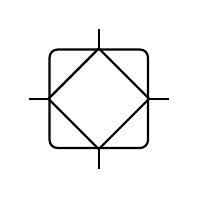
\begin{tikzpicture}[baseline=0]
      \node[contour] (t) {};
      \draw[index] (t.north) -- +(0,\tu);
      \draw[index] (t.east) -- +(\tu,0);
      \draw[index] (t.south) -- +(0,-\tu);
      \draw[index] (t.west) -- +(-\tu,0);
      \draw[index] (t.north) -- (t.east);
      \draw[index] (t.east) -- (t.south);
      \draw[index] (t.south) -- (t.west);
      \draw[index] (t.west) -- (t.north);
    \end{tikzpicture} 
  },
  4 \times
  {
    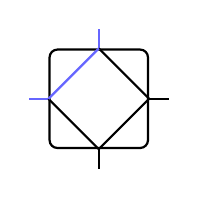
\begin{tikzpicture}[baseline=0]
      \node[contour] (t) {};
      \draw[highlight] (t.north) -- +(0,\tu);
      \draw[index] (t.east) -- +(\tu,0);
      \draw[index] (t.south) -- +(0,-\tu);
      \draw[highlight] (t.west) -- +(-\tu,0);
      \draw[index] (t.north) -- (t.east);
      \draw[index] (t.east) -- (t.south);
      \draw[index] (t.south) -- (t.west);
      \draw[highlight] (t.west) -- (t.north);
    \end{tikzpicture} 
  },
  4 \times
  {
    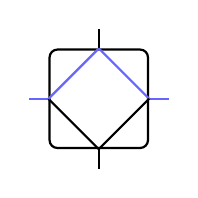
\begin{tikzpicture}[baseline=0]
      \node[contour] (t) {};
      \draw[index] (t.north) -- +(0,\tu);
      \draw[highlight] (t.east) -- +(\tu,0);
      \draw[index] (t.south) -- +(0,-\tu);
      \draw[highlight] (t.west) -- +(-\tu,0);
      \draw[highlight] (t.north) -- (t.east);
      \draw[index] (t.east) -- (t.south);
      \draw[index] (t.south) -- (t.west);
      \draw[highlight] (t.west) -- (t.north);
    \end{tikzpicture} 
  },
  2 \times
  {
    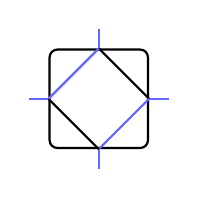
\begin{tikzpicture}[baseline=0]
      \node[contour] (t) {};
      \draw[highlight] (t.north) -- +(0,\tu);
      \draw[highlight] (t.east) -- +(\tu,0);
      \draw[highlight] (t.south) -- +(0,-\tu);
      \draw[highlight] (t.west) -- +(-\tu,0);
      \draw[index] (t.north) -- (t.east);
      \draw[highlight] (t.east) -- (t.south);
      \draw[index] (t.south) -- (t.west);
      \draw[highlight] (t.west) -- (t.north);
    \end{tikzpicture} 
  },
  4 \times
  {
    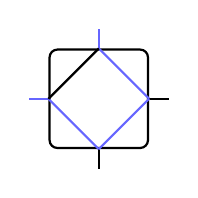
\begin{tikzpicture}[baseline=0]
      \node[contour] (t) {};
      \draw[highlight] (t.north) -- +(0,\tu);
      \draw[index] (t.east) -- +(\tu,0);
      \draw[index] (t.south) -- +(0,-\tu);
      \draw[highlight] (t.west) -- +(-\tu,0);
      \draw[highlight] (t.north) -- (t.east);
      \draw[highlight] (t.east) -- (t.south);
      \draw[highlight] (t.south) -- (t.west);
      \draw[index] (t.west) -- (t.north);
    \end{tikzpicture} 
  },
  {
    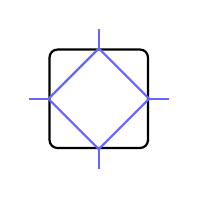
\begin{tikzpicture}[baseline=0]
      \node[contour] (t) {};
      \draw[highlight] (t.north) -- +(0,\tu);
      \draw[highlight] (t.east) -- +(\tu,0);
      \draw[highlight] (t.south) -- +(0,-\tu);
      \draw[highlight] (t.west) -- +(-\tu,0);
      \draw[highlight] (t.north) -- (t.east);
      \draw[highlight] (t.east) -- (t.south);
      \draw[highlight] (t.south) -- (t.west);
      \draw[highlight] (t.west) -- (t.north);
    \end{tikzpicture} 
  }
  \right\} .
\]
\item Some diagrams are
\begin{align*}
  {
    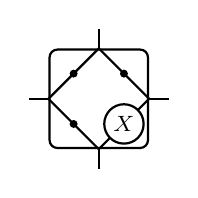
\begin{tikzpicture}[baseline=0]
      \node[contour] (t) {};
      \draw[index] (t.north) -- +(0,\tu);
      \draw[index] (t.east) -- +(\tu,0);
      \draw[index] (t.south) -- +(0,-\tu);
      \draw[index] (t.west) -- +(-\tu,0);
      \draw[index] (t.north) -- (t.east) node[site,midway]{};
      \draw[index] (t.east) -- (t.south) node[plain,midway]{$X$};
      \draw[index] (t.south) -- (t.west) node[site,midway]{};
      \draw[index] (t.west) -- (t.north) node[site,midway]{};
    \end{tikzpicture} 
  }
  &=
  {
    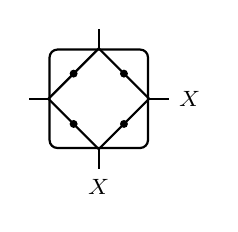
\begin{tikzpicture}[baseline=0]
      \node[contour] (t) {};
      \draw[index] (t.north) -- +(0,\tu);
      \draw[index] (t.east) -- +(\tu,0) node[right]{$X$};
      \draw[index] (t.south) -- +(0,-\tu) node[below]{$X$};
      \draw[index] (t.west) -- +(-\tu,0);
      \draw[index] (t.north) -- (t.east) node[site,midway]{};
      \draw[index] (t.east) -- (t.south) node[site,midway]{};
      \draw[index] (t.south) -- (t.west) node[site,midway]{};
      \draw[index] (t.west) -- (t.north) node[site,midway]{};
    \end{tikzpicture} 
  }, \quad
  {
    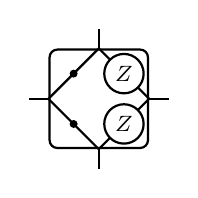
\begin{tikzpicture}[baseline=0]
      \node[contour] (t) {};
      \draw[index] (t.north) -- +(0,\tu);
      \draw[index] (t.east) -- +(\tu,0);
      \draw[index] (t.south) -- +(0,-\tu);
      \draw[index] (t.west) -- +(-\tu,0);
      \draw[index] (t.north) -- (t.east) node[plain,midway]{$Z$};
      \draw[index] (t.east) -- (t.south) node[plain,midway]{$Z$};
      \draw[index] (t.south) -- (t.west) node[site,midway]{};
      \draw[index] (t.west) -- (t.north) node[site,midway]{};
    \end{tikzpicture} 
  }
  =
  {
    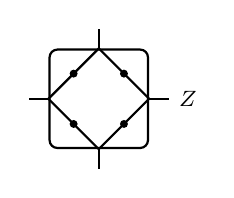
\begin{tikzpicture}[baseline=0]
      \node[contour] (t) {};
      \draw[index] (t.north) -- +(0,\tu);
      \draw[index] (t.east) -- +(\tu,0) node[right]{$Z$};
      \draw[index] (t.south) -- +(0,-\tu);
      \draw[index] (t.west) -- +(-\tu,0);
      \draw[index] (t.north) -- (t.east) node[site,midway]{};
      \draw[index] (t.east) -- (t.south) node[site,midway]{};
      \draw[index] (t.south) -- (t.west) node[site,midway]{};
      \draw[index] (t.west) -- (t.north) node[site,midway]{};
    \end{tikzpicture} 
  }, \\
  {
    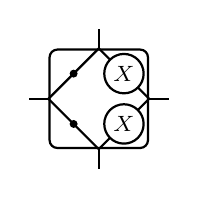
\begin{tikzpicture}[baseline=0]
      \node[contour] (t) {};
      \draw[index] (t.north) -- +(0,\tu);
      \draw[index] (t.east) -- +(\tu,0);
      \draw[index] (t.south) -- +(0,-\tu);
      \draw[index] (t.west) -- +(-\tu,0);
      \draw[index] (t.north) -- (t.east) node[plain,midway]{$X$};
      \draw[index] (t.east) -- (t.south) node[plain,midway]{$X$};
      \draw[index] (t.south) -- (t.west) node[site,midway]{};
      \draw[index] (t.west) -- (t.north) node[site,midway]{};
    \end{tikzpicture} 
  }
  &=
  {
    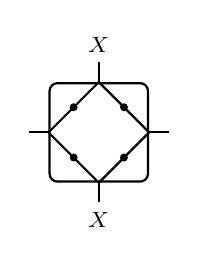
\begin{tikzpicture}[baseline=0]
      \node[contour] (t) {};
      \draw[index] (t.north) -- +(0,\tu) node[above]{$X$};
      \draw[index] (t.east) -- +(\tu,0);
      \draw[index] (t.south) -- +(0,-\tu) node[below]{$X$};
      \draw[index] (t.west) -- +(-\tu,0);
      \draw[index] (t.north) -- (t.east) node[site,midway]{};
      \draw[index] (t.east) -- (t.south) node[site,midway]{};
      \draw[index] (t.south) -- (t.west) node[site,midway]{};
      \draw[index] (t.west) -- (t.north) node[site,midway]{};
    \end{tikzpicture} 
  }\,, \quad
  {
    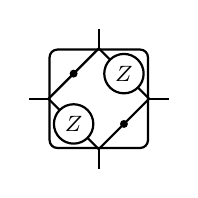
\begin{tikzpicture}[baseline=0]
      \node[contour] (t) {};
      \draw[index] (t.north) -- +(0,\tu);
      \draw[index] (t.east) -- +(\tu,0);
      \draw[index] (t.south) -- +(0,-\tu);
      \draw[index] (t.west) -- +(-\tu,0);
      \draw[index] (t.north) -- (t.east) node[plain,midway]{$Z$};
      \draw[index] (t.east) -- (t.south) node[site,midway]{};
      \draw[index] (t.south) -- (t.west) node[plain,midway]{$Z$};
      \draw[index] (t.west) -- (t.north) node[site,midway]{};
    \end{tikzpicture} 
  }
  =
  {
    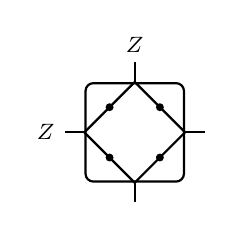
\begin{tikzpicture}[baseline=0]
      \node[contour] (t) {};
      \draw[index] (t.north) -- +(0,\tu) node[above]{$Z$};
      \draw[index] (t.east) -- +(\tu,0);
      \draw[index] (t.south) -- +(0,-\tu);
      \draw[index] (t.west) -- +(-\tu,0) node[left]{$Z$};
      \draw[index] (t.north) -- (t.east) node[site,midway]{};
      \draw[index] (t.east) -- (t.south) node[site,midway]{};
      \draw[index] (t.south) -- (t.west) node[site,midway]{};
      \draw[index] (t.west) -- (t.north) node[site,midway]{};
    \end{tikzpicture} 
  }
  =
  {
    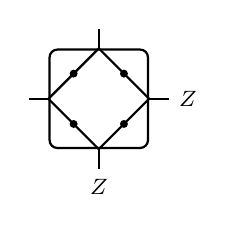
\begin{tikzpicture}[baseline=0]
      \node[contour] (t) {};
      \draw[index] (t.north) -- +(0,\tu);
      \draw[index] (t.east) -- +(\tu,0) node[right]{$Z$};
      \draw[index] (t.south) -- +(0,-\tu) node[below]{$Z$};
      \draw[index] (t.west) -- +(-\tu,0);
      \draw[index] (t.north) -- (t.east) node[site,midway]{};
      \draw[index] (t.east) -- (t.south) node[site,midway]{};
      \draw[index] (t.south) -- (t.west) node[site,midway]{};
      \draw[index] (t.west) -- (t.north) node[site,midway]{};
    \end{tikzpicture} 
  }\, .
\end{align*}
\item The $\mathrm{Z}_2$ invariance means that on the index level
\[
    {
    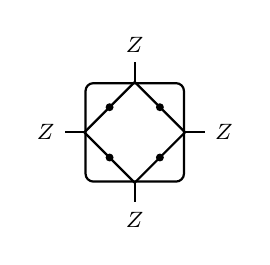
\begin{tikzpicture}[baseline=0]
      \node[contour] (t) {};
      \draw[index] (t.north) -- +(0,\tu) node[above]{$Z$};
      \draw[index] (t.east) -- +(\tu,0) node[right]{$Z$};
      \draw[index] (t.south) -- +(0,-\tu) node[below]{$Z$};
      \draw[index] (t.west) -- +(-\tu,0) node[left]{$Z$};
      \draw[index] (t.north) -- (t.east) node[site,midway]{};
      \draw[index] (t.east) -- (t.south) node[site,midway]{};
      \draw[index] (t.south) -- (t.west) node[site,midway]{};
      \draw[index] (t.west) -- (t.north) node[site,midway]{};
    \end{tikzpicture} 
  }
  =
  {
    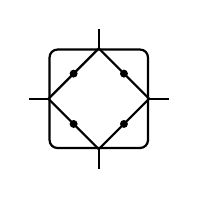
\begin{tikzpicture}[baseline=0]
      \node[contour] (t) {};
      \draw[index] (t.north) -- +(0,\tu);
      \draw[index] (t.east) -- +(\tu,0);
      \draw[index] (t.south) -- +(0,-\tu);
      \draw[index] (t.west) -- +(-\tu,0);
      \draw[index] (t.north) -- (t.east) node[site,midway]{};
      \draw[index] (t.east) -- (t.south) node[site,midway]{};
      \draw[index] (t.south) -- (t.west) node[site,midway]{};
      \draw[index] (t.west) -- (t.north) node[site,midway]{};
    \end{tikzpicture} 
  }\, .
\]
\item Using the properties above one easily checks that $A_v \ket{\Psi} = \ket{\Psi}$.
Then, we can check $B_p \ket{\Psi} = \ket{\Psi}$, since
\[
  {
    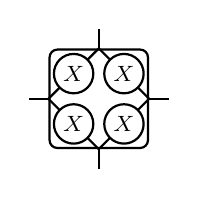
\begin{tikzpicture}[baseline=0]
      \node[contour] (t) {};
      \draw[index] (t.north) -- +(0,\tu);
      \draw[index] (t.east) -- +(\tu,0);
      \draw[index] (t.south) -- +(0,-\tu);
      \draw[index] (t.west) -- +(-\tu,0);
      \draw[index] (t.north) -- (t.east) node[plain,midway]{$X$};
      \draw[index] (t.east) -- (t.south) node[plain,midway]{$X$};
      \draw[index] (t.south) -- (t.west) node[plain,midway]{$X$};
      \draw[index] (t.west) -- (t.north) node[plain,midway]{$X$};
    \end{tikzpicture} 
  }
  =
  {
    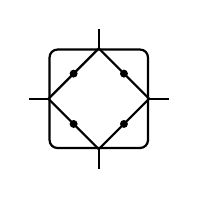
\begin{tikzpicture}[baseline=0]
      \node[contour] (t) {};
      \draw[index] (t.north) -- +(0,\tu);
      \draw[index] (t.east) -- +(\tu,0);
      \draw[index] (t.south) -- +(0,-\tu);
      \draw[index] (t.west) -- +(-\tu,0);
      \draw[index] (t.north) -- (t.east) node[site,midway]{};
      \draw[index] (t.east) -- (t.south) node[site,midway]{};
      \draw[index] (t.south) -- (t.west) node[site,midway]{};
      \draw[index] (t.west) -- (t.north) node[site,midway]{};
    \end{tikzpicture} 
  }\,,
\]
One should also check the plaquette between 4 tensors, and using the properties in (b) to show invariance.

\item 
The string $W_l^{(e)}$ generates a series of $X$ matrices in between the tensors, along the path $l$.
They all cancel out, except at the endpoint, where we have a new tensor 
\[
  B^{i_1,i_2,i_3,i_4}_{\alpha,\beta,\gamma,\delta} = \sum X_{\delta,\delta^\prime} A^{i_1,i_2,i_3,i_4}_{\alpha,\beta,\gamma,\delta^\prime} .
\]
Notice that $Z^{\otimes 4} B^i = -B^i$.
The $W_{l^*}^{(m)}$ acts with $Z$ on the physical level, generating a string of $Z$s on the virtual level. Notice that this string can be moved at will, except for the endpoints, where we have a new tensor
\[
  C^{i_1,i_2,i_3,i_4}_{\alpha,\beta,\gamma,\delta} = \sum Z_{i_4,i_4^\prime} A^{i_1,i_2,i_3,i_4^\prime}_{\alpha,\beta,\gamma,\delta} .
\]
This tensor remains invariant under the symmetry: $Z^{\otimes 4} C^i = C^i$.
\item From the structure of the tensors, we see that a non-zero term in the contraction of the tensor network corresponds to a closed loop configuration. 
Since there is a one-to-one correspondence between the physical indices $i_1,\dots,i_4$ of the tensors and the lattice sites, we conclude that there is a bijection between a non-zero tensor contraction term and a loop configuration, meaning the tensor network corresponds to the ground state of the toric code.
\end{enumerate}
\end{section}

\begin{section}{}
No solution is presented for this exercise.
\end{section}
\end{document}
%%%%%%%%%%% Here Ends Document %%%%%%%%%%
